% CREATED BY MAGNUS GUSTAVER, 2020
\chapter{Background} \label{Theory}
%This section presents theory used in this thesis. It starts with the hardware used to enable autonomous flight of the drone, then the software and how communication between the computer and the phone is handled.

In this chapter, the foundation on which the implementation and results are built upon are presented. The chapter begins with an overview of the drone hardware, followed by an explanation of the software. This includes the drone's flight control, communication with ATOS, object detection and tracking as well as limitations pertaining to every component.

\section{Hardware} \label{Hardware}
In this section, the hardware used will be presented which is a drone, a mobile device and the test objects. 

\subsection{DJI Mavic 2 Enterprise Zoom} \label{DJI}
The unmanned aerial vehicle (UAV) that was used in this project was the DJI Mavic 2 Enterprise, developed by the Chinese technology company DJI, seen in Fig. \ref{fig:drone}.
\begin{figure}[h!]
\centering
 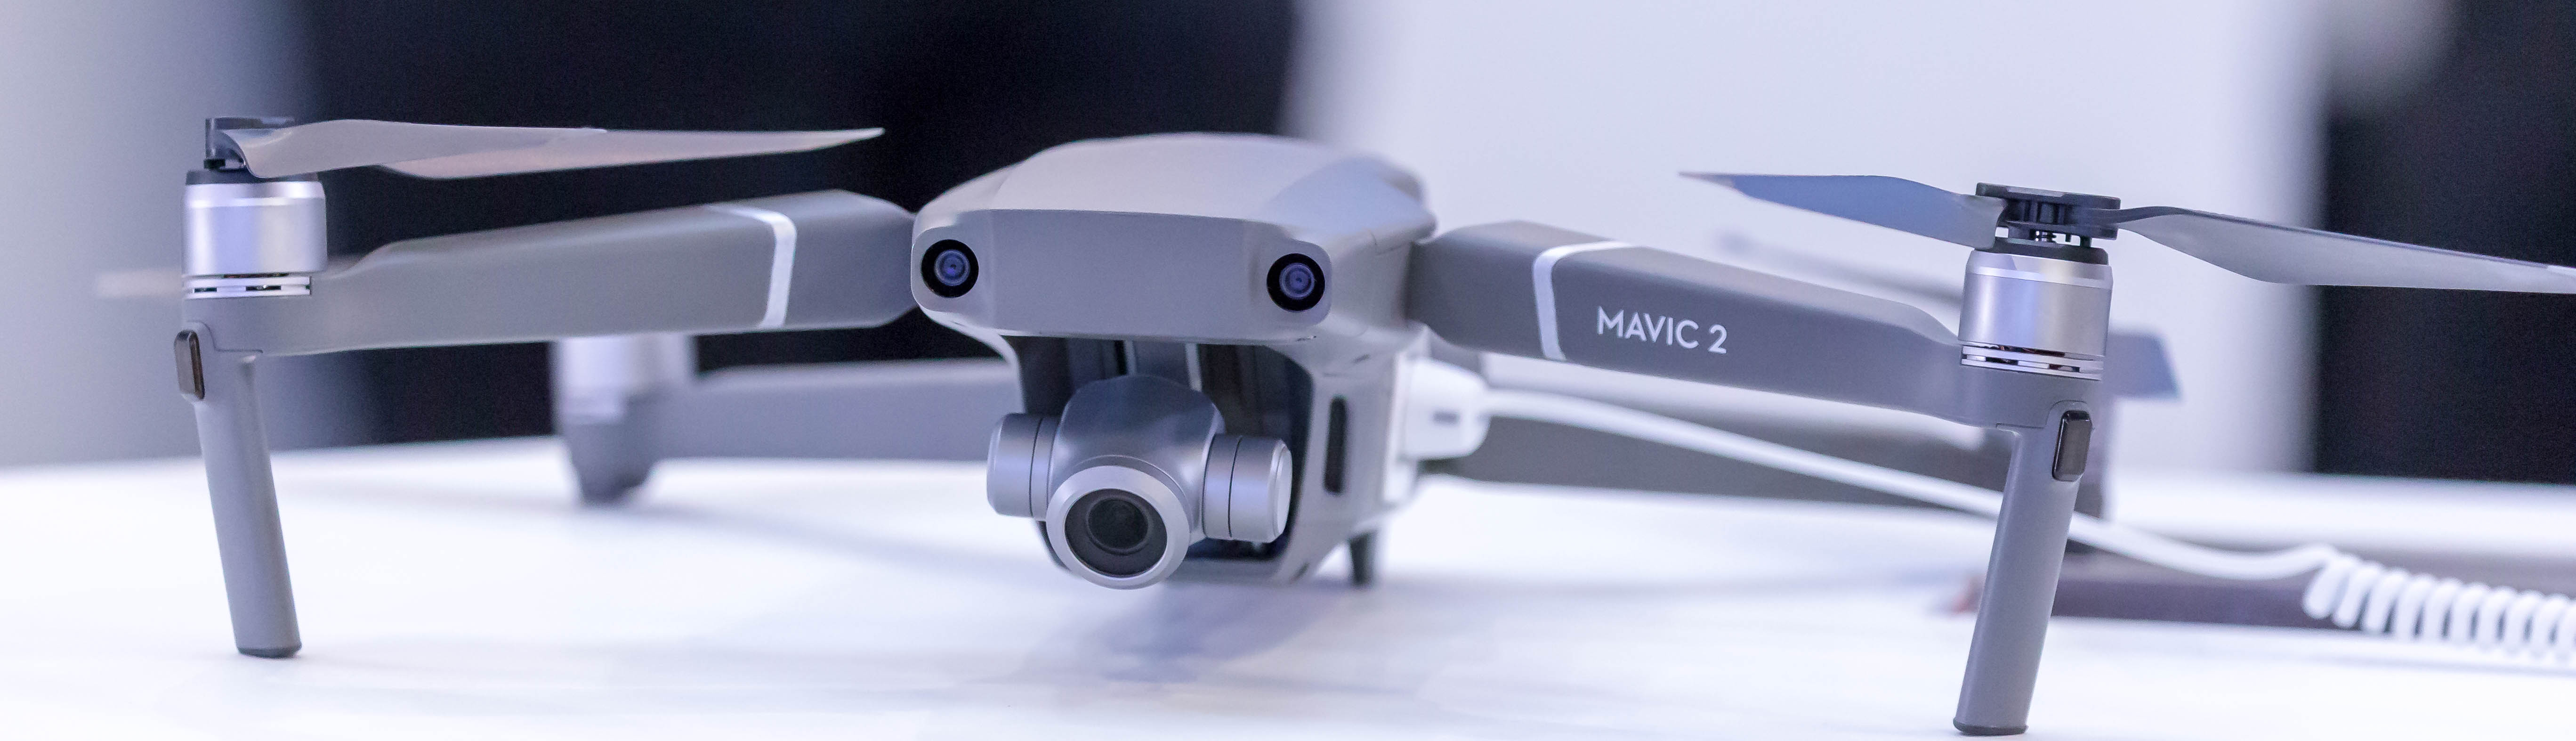
\includegraphics[width=\textwidth,angle =0]{figure/bild_på_drönare.jpg}
\caption{Picture of the DJI Mavic 2 Enterprise. Source~\cite{Verc2018Close-upDrone}. CC-BY 2.0}
\label{fig:drone}
\end{figure}
\newline
The Mavic 2 Enterprise is equipped with a 3-axis gimbal-stabilized camera that can capture high-quality 4K video and 12MP photos~\cite{DJI2018MavicDJI}. The gimbal is able to be controlled by both software and manual inputs to the remote controller. It also features omnidirectional obstacle sensing and avoidance with sensors positioned on the front, back, bottom, and sides, as well as a GPS and magnetometer sensor, which allows the drone to maintain a stable hovering position.
\newline

%\textcolor{red}{Ska detta vara med? In order to control the drone, an RC is necessary, which communicates with the drone on 2.4GHz or 5.8GHz depending on the surroundings.}
The Mavic 2 Enterprise has a maximum flight time of up to 31 minutes and a range of up to 10 km~\cite{DJI2018MavicDJI}, making it a versatile and effective tool for various applications. Yet, drone laws and regulations vary by country and region, and certain areas may require permits to fly beyond visual line of sight or certain distances. Therefore, strict adherence to local regulations and safety protocols was of paramount importance when operating the Mavic 2 Enterprise or any other UAV. More on the rules and regulations of drone flight can be found in Sec.~\ref{Laws and rules}.
\newline 
\\

The drone came with a remote controller (RC), which could be connected to a compatible smartphone with a designated application via a USB-cable, as seen in Fig.~\ref{RC w phone}. This is required if a live feed from the drone's camera is desired. DJI offers its own application that offers drone operators a wide array of modes, settings, and options to customize and monitor the live feed from the drone. This application can be downloaded from either the App Store or Google Play. However, the group had to establish a connection with the existing in-house software ATOS, outlined in Sec.~\ref{ATOS} to execute the tests. Since the ATOS software is not used outside of AstaZero, DJI offered no easy integration with ATOS. The scope of the project was therefore much more specific compared to what the demo application offers and accordingly, a new application needed to be developed.

\begin{figure}[!h]
\centering
 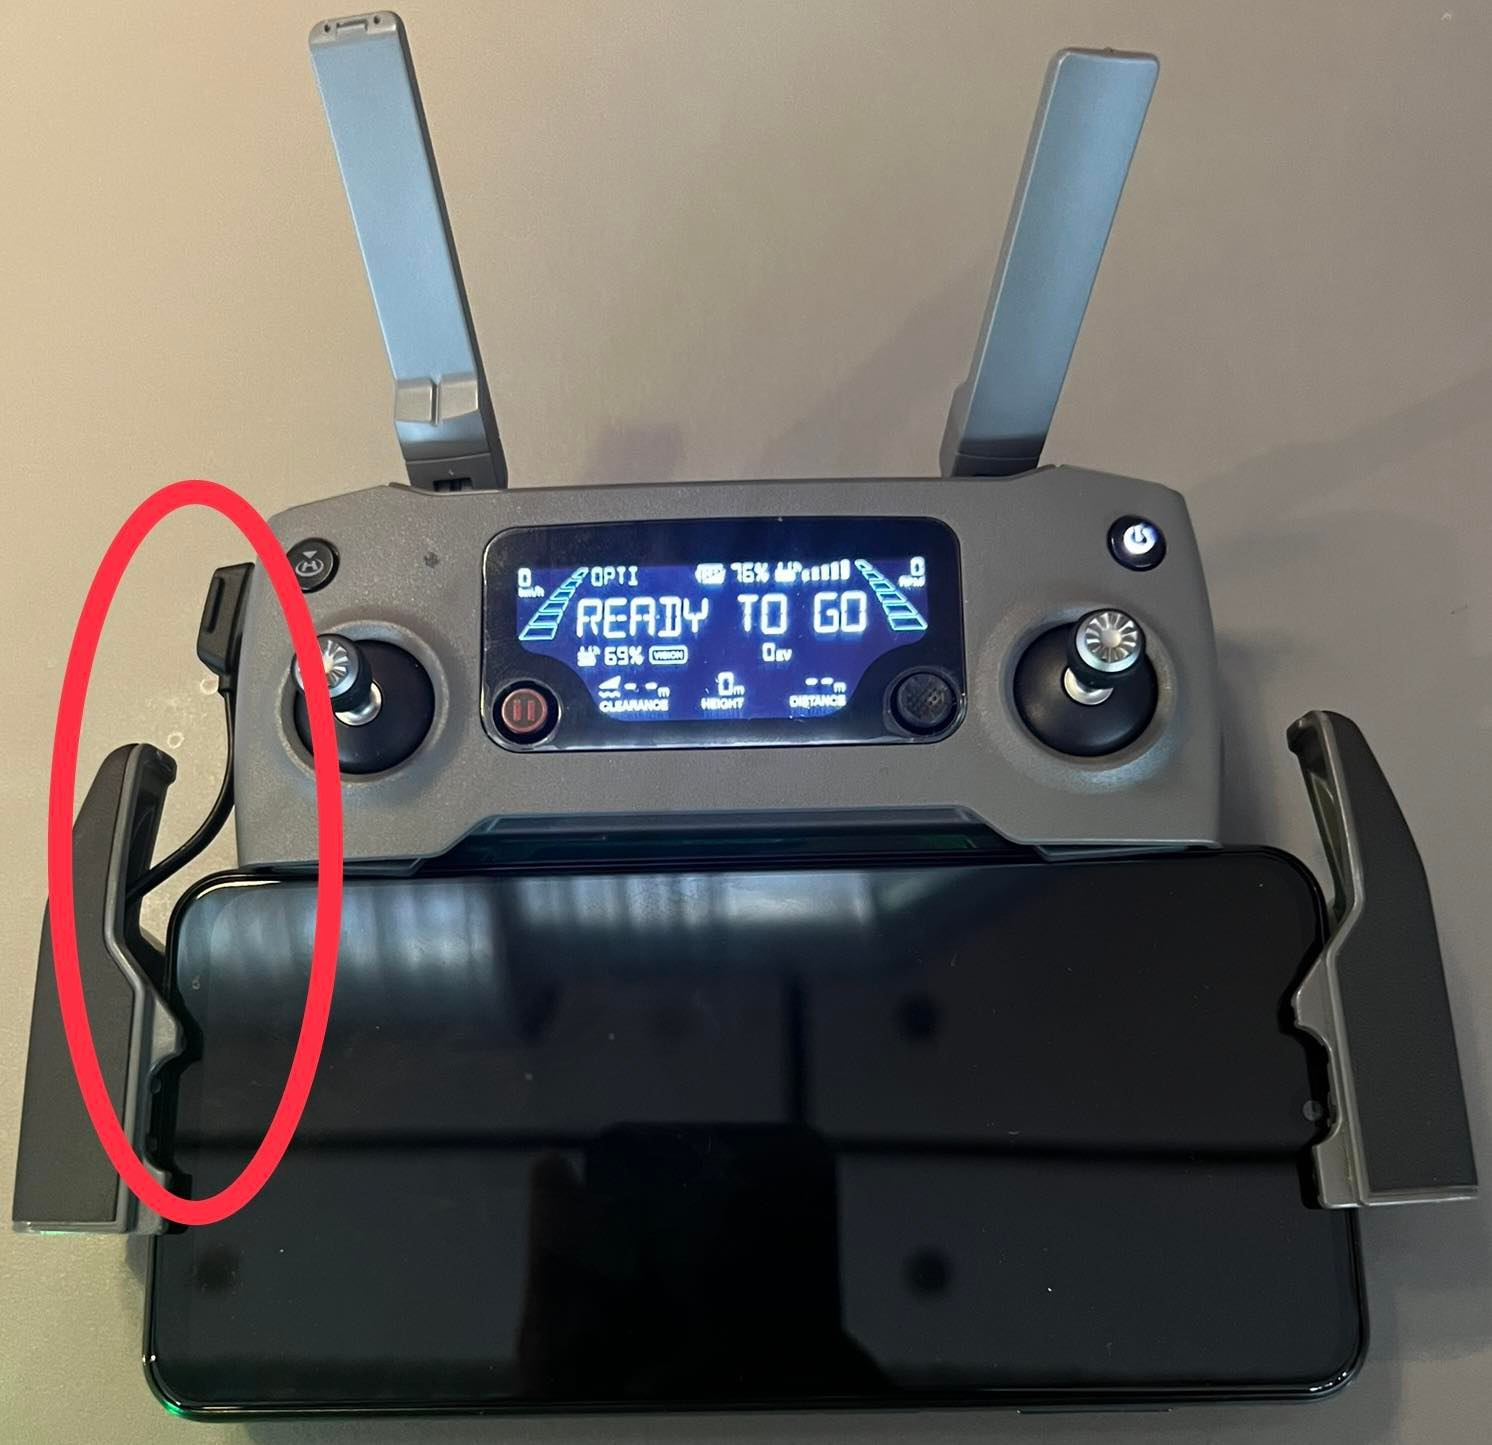
\includegraphics[width=0.65\textwidth,angle =0]{figure/345858277_6148140848602054_316699155434135194_n.jpg}
\caption{Picture of the mobile device connected to the RC via an USB cable (highlighted in red). Source: Primary}
\label{RC w phone}
\end{figure}


\subsection{Samsung A13} \label{Samsung}
The Samsung Galaxy A13 is the mobile device developed by Samsung. The device comes equipped with the Exynos 850 chipset, which is a mobile processor that provides great computing capabilities \cite{a13_chipset} on mobile devices as well as facilitating fast mobile internet. It is compatible with networks ranging from 2G to LTE with downlink speeds of up to 300Mbps and uplink speeds of up to 150Mbps. The model of the A13 device which was provided by AstaZero has the Android 12 operating system and comes with 64GB of internal storage, 4GB of RAM and a 5,000mAh battery. 
\\ \\
In summary, the Samsung A13 mobile device is a suitable choice for the current application when not performing any other tasks in parallel. It is a reliable and cost-effective device with more than sufficient capabilities, whilst running the correct operating system for the project. See Fig.~\ref{fig:samsung_a13} for an external view of the A13 device.  

\begin{figure}[h!]
\centering
 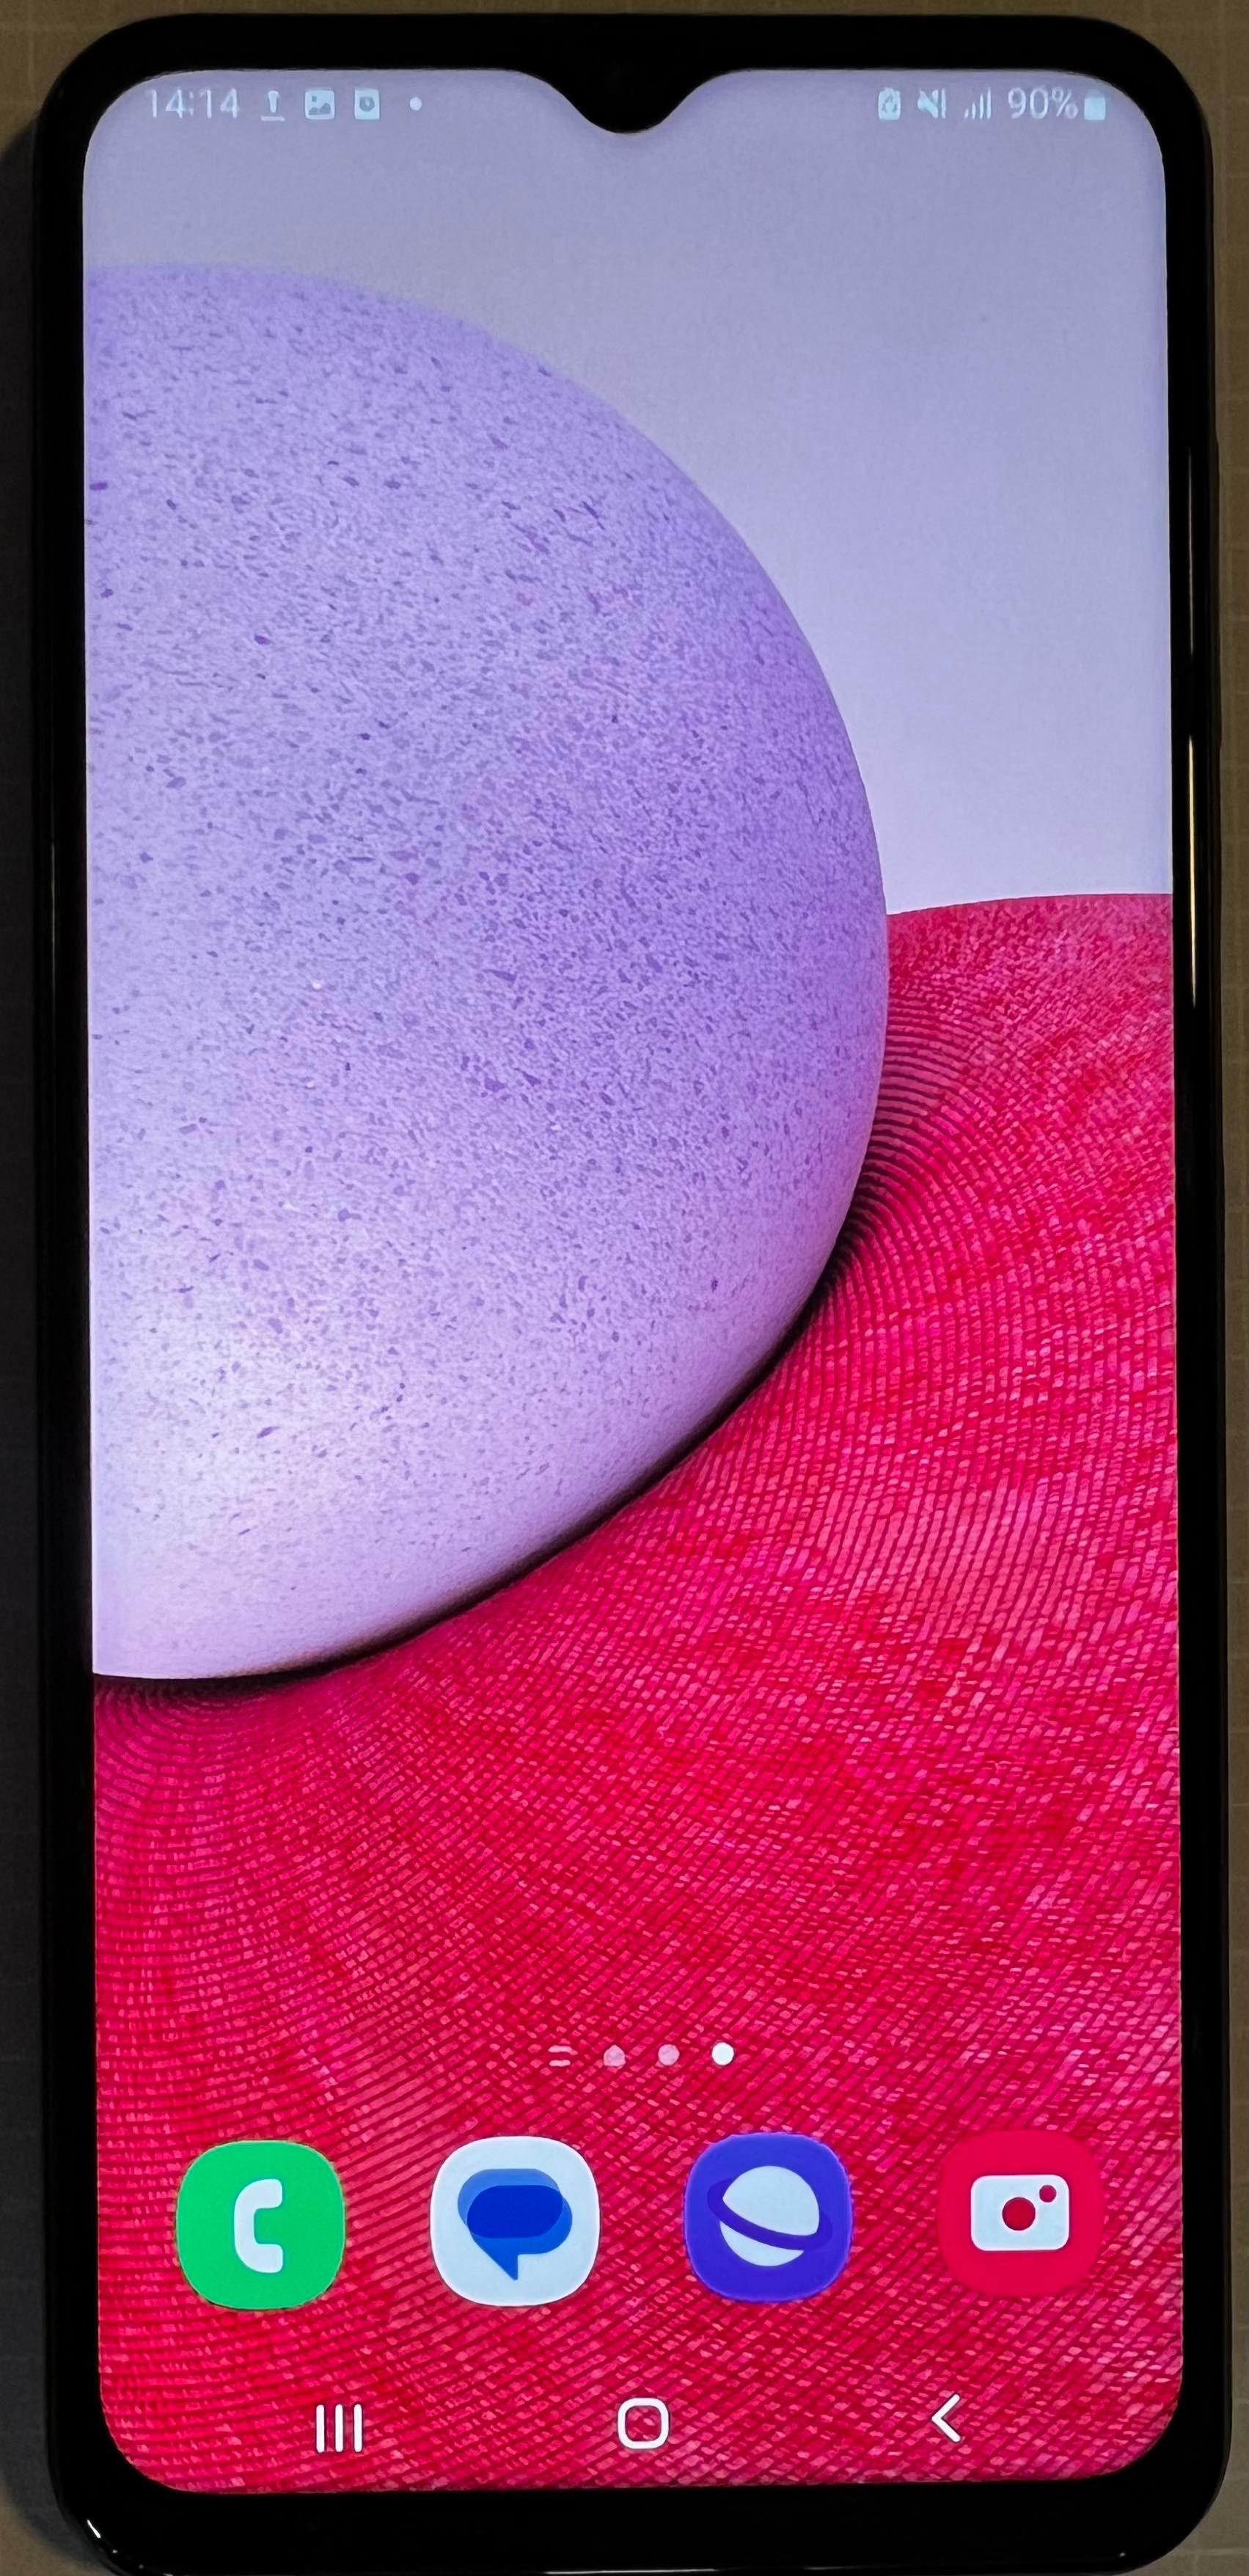
\includegraphics[width=0.35\textwidth,angle =270]{figure/345610209_239776231969766_5365333810102475276_n.jpg}
\caption{Picture of the Samsung A13. Source: Primary}
\label{fig:samsung_a13}
\end{figure}


\section{Software} \label{Software}
This section will provide an overview of the software utilized in this project. The key components; ATOS, Linux and Ubuntu 20.04 as the operating system, along with essential applications such as Java, Android SDKs, and Android Studio. Additionally, the project incorporates DJI Waypointmission, AstaZero's application, object detection, a tracking algorithm, and a Graphical User Interface (GUI).

\subsection{Autonomous Vehicle testing operating system (ATOS)} \label{ATOS}
The core of each test is ATOS, short for Automatic Vehicle Testing Operating System, which follows the standards stated in the ISO22133 documentation~\cite{iso22133} and creates trajectories for each object that is part of the test. An extensive comprehension of the ATOS software needed to be obtained, which included the functional requirements, software specifications and the communication protocol. The information can be obtained from the ISO22133 protocol as well as in the actual code-base~\cite{AstaZero2023ATOS:Systems.}. ATOS is mainly written in C and C++ and developed on a Linux machine. The integration of ATOS in this project is illustrated in Fig.~\ref{fig:ATOS-flow}.
\begin{figure}[H]
  \centering
  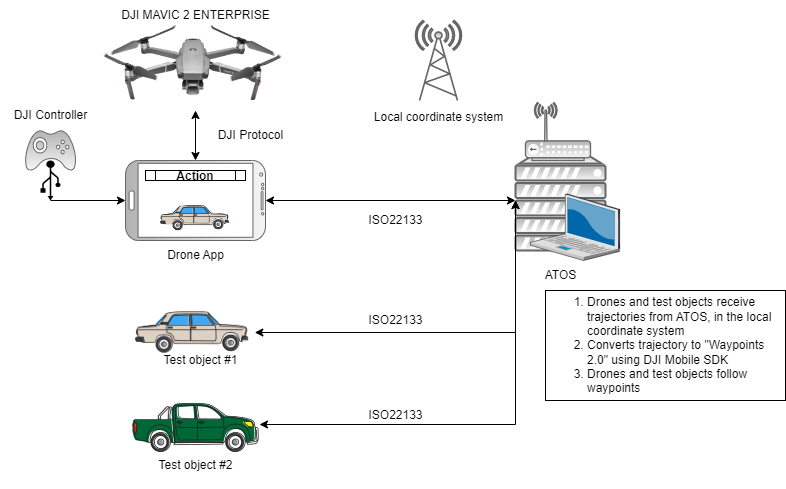
\includegraphics[width=\columnwidth]{figure/flow_config.png}
  \caption{ATOS integration with other objects. Source: Primary}
  \label{fig:ATOS-flow}
\end{figure}
Fig.~\ref{fig:iso_states} displays the various states and transitions that ATOS sends to all objects during a test, each representing a specific action. In the ``Init'' state, each object is initialized but not connected to ATOS. When ATOS establishes a successful connection, the connected objects moves to the ``Disarmed'' state, meaning it is ready to receive telemetry data and begin mission planning. Once ATOS transitions to ``Armed'', the objects receives the telemetry data and is set to execute the test. When ``Armed'', ATOS can start the test and the state will transition to ``Running'', which means that all objects follow their predetermined trajectories until each object reaches its endpoint. ATOS then moves to the ``Normal Stop'' state, indicating that the test has concluded. From ''Normal Stop,'' the objects can transition back to the ``Disarmed'' state to wait on a new trajectory. Additionally, the ``Disarmed'' state can be reached from the ``Emergency Stop'' state, which acts as a kill switch to abort the test.

\begin{figure}[h!]
  \centering
  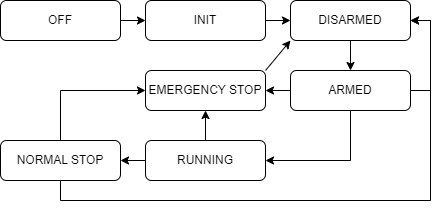
\includegraphics[scale=0.6]{figure/ISO-states.png}
  \caption{Illustration of relevant object states and their transitions. Source: Primary}
  \label{fig:iso_states}
\end{figure}
Note that some states from the ISO22133 protocol are not shown in the figure, as they are not relevant to this project. One such state is the ``Remote Ctl'' state, which allows the operator to move the object freely without relying on predetermined telemetry, while still maintaining a connection to the control center.

\subsection{AstaZero's application} \label{AZ's app}
AstaZero provided an application that they had begun working on~\cite{azGithubMobil}. The application included a DJI demo which was copied from DJI's publicly available demo applications~\cite{githubmobilesdk}. This application provided the basic functionality to connect and communicate with the drone, as well as two different components. These two components utilized a map to place waypoints and fly the mission.
\subsection{ISO DTS 22133 Communications Protocol} \label{ISO}
To conduct a thorough assessment of collision avoidance systems and perform various other tests, it was essential to carry out testing on specialized proving grounds. These proving grounds provided a controlled environment that ensured the safety of both the driver and other motorists.
\\

In order to create realistic traffic scenarios during testing, the proving grounds had to utilize various targets that represented both vehicles and pedestrians. These targets helped simulate different scenarios that could occur on the road, enabling a comprehensive evaluation of the collision avoidance systems.
\\ \\
The ISO DTS 22133 standard~\cite{iso22133} describes requirements, functionality, and protocol necessary for controlling multi target-carrier systems to create and monitor realistic traffic scenarios in a safe and effective manner. The ISO22133 is a standard designed to work with multiple manufacturers and different test objects. Each object holds a state that is controlled by ATOS, as described in Sec.~\ref{ATOS}, and the protocol is used to communicate this to all relevant objects. It also facilitates the communication of position, speed and heading from ATOS to the test object in question.

\subsection{Linux and Ubuntu 20.04} \label{Linux}
As stated in Sec.~\ref{ATOS}, ATOS was developed using a Linux operating system, specifically Ubuntu 20.04. Linux and Windows have some fundamental differences making it impossible to compile the necessary projects aimed at Linux operating systems on Windows. Both the ATOS project and the Android application provided by AstaZero have dependencies on other Linux programs which is why an old version of the Ubuntu operating system was required.

\subsection{Java, Android, SDKs and Android Studio} \label{Java, Android....}
The application was built on top of one of the major mobile operating systems named Android. Android provides a framework for communicating with any mobile device running the Android system making the development not tied to one specific device, but rather any device capable of running Android. 
\\ \\
All Android applications are constructed using activities, which serve as the fundamental elements of the application's user interface. Activities act as individual screens or windows that facilitate user interaction within the application~\cite{Android}. Each activity functions as an independent component, possessing its own life cycle. It can be initiated, halted, and terminated autonomously from other activities within the application. Activities also have the capability to communicate with one another, allowing for the sharing of information among all components of an application. Additionally, based on the provided information, new activities can be created when required.
\\ \\
For instance, within the confines of this project, one activity could be the first page displayed, e.g. the landing page, while another activity could be the interface that displays drone information. Together these different activities make up the application and communicate with each other.
\\ \\
The recommended option to develop Android applications is Android's own integrated development environment (IDE) called Android Studio. The program provides all the necessary tools for developing Android applications in Java. It also has support for designing user interfaces in both a manual way using the markup language XML or a via drag-and-drop functionality.
\\ \\
Android enables developers to use outside libraries, also called Software Development Kits (SDK). These external libraries allows the developer to use code written by other developers and use their frameworks. DJI provides their own SDK for communicating with their different products.
\\ \\
To access the functionalities of the DJI Mavic 2 Enterprise drone, a mobile application must be connected to the drone's remote controller (RC). DJI's framework for Android devices enables users to access functions such as reading drone states, initiating or terminating video recording, obtaining a live feed from the drone's camera, land at a given point and starting or stopping the motors. DJI's website~\cite{githubmobilesdk} contains tutorials on how to implement various types of functions for the application. This has served as a foundation for learning how to communicate with the drone. Moreover, GitHub hosts a diverse range of projects of varying kinds that have been explored to acquire knowledge of the DJI Mobile SDK API.

\subsection{DJI WaypointMission}
The drone is able to fly on its own with different protocols provided by the DJI SDK. One of these protocols is the WaypointMission~\cite{WaypointMission}, which enables the developer to create a list of geographical locations to which the drone will fly. The developer can control the speed, heading, latitude, and longitude that the drone should have at each waypoint. It also offers a callback for different events such as mission start, waypoint reached, and mission uploaded. This can be used to perform different actions based on the state of the mission. 

\subsection{Object detection} \label{sec:Obj_detextion}
In order to ensure that the camera captures the vehicles at the optimal angle, it was imperative for the drones to accurately detect the location of the cars as the drones followed them. 
\\ \\
Object detection is a rapidly developing field of computer vision that has gained significant attention in recent years. At its core, object detection involves the automatic identification and classification of objects within digital images. This is accomplished through the use of sophisticated algorithms that are designed to recognize specific patterns and features within the image data.
\\

According to Myeongsuk and Sanghoon~\cite{Pak2018ARecognition}, the process of image recognition is typically achieved using deep learning algorithms, such as convolutional neural networks (CNNs). These networks consist of several layers, including convolutional, pooling, and fully connected layers, which work together to extract and analyze features from the input image. The Single-shot Multibox Detection model~\cite{ssd} that TensorFlow Lite offers~\cite{tflite} does classification using convolutional layers instead of fully connected ones. 

\subsubsection{TensorFlow Lite}
TensorFlow Lite is a specialized library designed specifically for mobile applications, offering pre-trained models for various scenarios, including object detection~\cite{tflite}. Given a mobile device's limited processing power compared to a traditional computer, TensorFlow Lite models are compressed versions of their normal TensorFlow counterparts, possessing less complexity.
Thus, a TensorFlow Lite model trades a small amount of accuracy for significantly improved computational speed compared to a normal TensorFlow model, making it well-suited to our goal of running such a model on a mobile device.

\subsubsection{Convolutional layers in CNNs} 
Convolutional layers are typically the first few layers in a CNN~\cite{cnnforklarning}, meaning they are the first to receive the input image. When images are used as input, they are typically treated as matrices of pixel values. Pixels in grayscale images can be represented by a value between 0 and 1, where 0 is black, and 1 is white. The image is subsequently transformed into a numerical representation to which mathematical operations can be applied. In CNNs, said operation is the dot product between the filter and the grid of pixel values the filter applies to. The result of the dot product replaces the pixel value in the feature map produced by the CNN.
\\ \\
CNNs have a parameter called stride, which determines how many pixels the filter is moved by after it has been applied to a pixel. Given a stride of 1, the filter will be applied to each pixel, with the filter first being applied to every pixel in the top row, followed by every pixel in the second top row. Given a stride of 2, the filter will be applied to every other pixel in the first row, then every other pixel in the third. The height and width of the output, a feature map, are thereby halved.
\\ \\
Pixels in color images can not be represented by a single value like pixels in grayscale images; they can, however, be represented by three values, the level of red, green, and blue present in the pixel. The image is therefore turned into three $w\cdot h$ matrices where $w$ is the width, and h is the height of the image in pixels. The values in the first matrix indicate the level of red present in each pixel of the image, the values of the second matrix indicate the level of green present in each pixel, and the values in the third matrix indicate the level of blue present in each image. A three-dimensional filter can be used to apply a filter to the whole image, meaning all three matrices. 
\\ \\
The outputted feature map of a CNN highlights a specific feature. In Fig.~\ref{fig:conv}, diagonal features in the shown direction are highlighted in the resulting feature map. To highlight more complex patterns, feature maps can be used as inputs to other convolutional layers. Consecutive convolutional layers are usually used in CNN:s.


\begin{figure}[H]
  \centering
  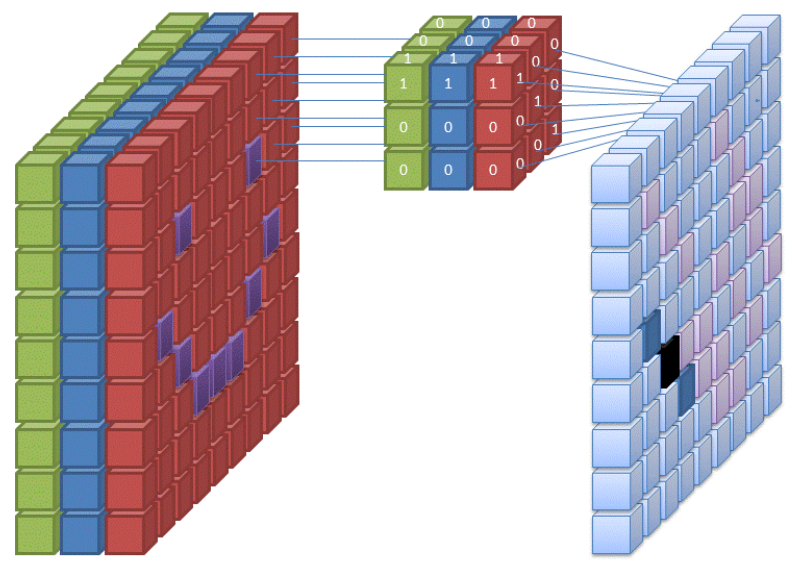
\includegraphics[width=\columnwidth]{figure/convlayer.png}
  \caption{A convolutional layer is applied to an image, resulting in a feature map. Source: \cite{cnnbild}. CC-BY SA 4.0}
  \label{fig:conv}
\end{figure}

\subsubsection{Pooling layers in CNNs}
Various pooling layers exist, including max and average pooling layers, which operate similarly but employ distinct functions for selecting representative values~\cite{cnnforklarning}. Max pooling is a layer in CNNs often used in combination with convolutional layers. A max-pooling layer reduces the size of an image or matrix by splitting it into grids and representing each grid by the largest value in that grid. The features highlighted by previous convolutional layers are preserved by keeping the highest values of a grid. Since the image size gets reduced by the max pooling layer and certain features are highlighted, patterns of varying sizes can be detected. Filters applied to the image in its original resolution can detect local, smaller features, and filters applied to the image after a couple of max pooling layers can detect more global features since more of the image fits in the filter. Reducing the resolution of an image also boosts computing efficiency.

%\subsubsection{Fully connected layers in CNNs}
%Fully connected layers are the parts of CNNs that can learn to interpret patterns and classify those patterns. The input or inputs to fully connected layers are the feature maps generated by the convolutional and max pooling layers that precede them in CNNs. The learning process for fully connected layers is a complex process called backpropagation which compares the model's outputted class to some training data with the actual class of the image. By comparing the actual output with the expected output, the parameters of the model can be tweaked to generate a better prediction to the training data. Given enough training data, layers and neurons in those layers a neural network has been shown to be able to approximate any function 

\subsubsection{Single-shot Multibox Detection}
\label{ssdbackground}
A popular model used for object detection is Single-shot Multibox Detection (SSD)~\cite{ssd}. An SSD is a type of CNN used for object detection. The initial part of the SSD architecture consists of convolutional and max pooling layers. These can be derived from existing image classifier models. Since these layers use max pooling layers and the image's resolution is gradually decreased, the feature maps produced can highlight different features of differently sized objects. The next part of the SSD uses the feature maps generated by this first part of the SSD to predict bounding boxes, the rectangle surrounding a detected object. The bounding boxes are classified, and the model removes duplicate objects. Both the bounding box prediction and classification are done using convolutional layers. The output consists of a list of detected objects. Each object has a class, a size and position of the bounding box surrounding it, and a confidence score of how certain the model is of the prediction. An SSD is considered a good model for real-time object detection because of its computational efficiency and speed. The initial part of the SSD architecture, which can be derived from an existing image classifier, can be selected to achieve an optimal trade-off between accuracy and computational efficiency~\cite{mobilenet}
\\ \\
One model that is able to utilize the SSD is a stripped version of the MobileNet model~\cite{mobilenet}. This model contains many layers, but removing the fully connected layers leads to the model being a good option for image classification for mobile devices. MobileNet is a lightweight model that still performs comparably well and has substantially fewer parameters compared to alternative models, making it suitable for object detection on a mobile device.

\subsection{Tracking Algorithm} \label{Tracking algorithm}

Object detection is a crucial process for identifying specific objects within an image or video frame. However, object tracking takes this process to the next level by not only identifying the objects but also monitoring their movement over time. To facilitate this transition, one of the most widely-used approaches is implementing an algorithm that can trace the identified objects from frame to frame. This is achieved by employing a tracking algorithm that uses the number of objects as well as their positions, heading and speed to track the different objects.

\subsection{Graphical User Interface (GUI)}\label{GUI}
Developing the GUI for the application included designing a functional and informative interface. The interface was developed to be easy to use while also providing all the necessary information and controls for the operator and capturing the footage. Below are some scientifically based~\cite{AntchevaGUIDELINESGUI}, as well as some project-based, considerations used for the GUI-development. 
\\

\begin{itemize}
    \item \textbf{Creating a user centered interface:} The GUI should be intuitive and easy to navigate. 
    \item \textbf{Include all necessary commands:} Evaluate what commands are needed for executing the program and make them easily accessible. 
    \item \textbf{Create a distinct visual hierarchy:} Prioritize important information and make it easy for the user to locate the necessary information. 
    \item \textbf{Real-time representation:} The GUI should provide users with the real-time footage captured by the drone, as well as real-time updates of the drones battery life etc. 
    
\end{itemize}

\section{Limitations} \label{Limitations}
This section will delineate the limitations associated with the utilization of the drone hardware, the DJI SDK application with heavy focus in the WaypointMission software as well as the already existing code base. 

\subsection{Hardware} \label{Drone limitations}
Research into the limitations of the drone presented in Sec.~\ref{DJI} was needed to obtain necessary information on the feasibility of achieving the performance requirements. The physical limitations does not hinder the project potential as much as the software limitations described in Sec.~\ref{limits of dji sdk}. This assumption is purely based on the fact that Euro NCAP tests chosen for this project do not create an environment that pushes the limits of the drone capabilities~\cite{DJI2021MAVICMANUAL} from a hardware standpoint. Even though the drone hardware limitations, for this specific test, see Sec.~\ref{sec:project outline}, does not become a problem, it is worth noting that there exists Euro NCAP tests~\cite{speed_euro_ncap} with speeds that exceed the speed capability of the drone~\cite{DJI2021MAVICMANUAL}.
\\ \\
Furthermore, the computing power of the Samsung A13 phone presented in Sec.~\ref{Samsung} will be significantly limited in terms of performance compared to a desktop or laptop computer. This limitation will become evident when performing tasks that require significant computational power, such as object detection and image recognition algorithms. Despite these limitations, with an appropriately streamlined software, the Samsung A13 could still provide a sufficient level of computational power for on-the-go image recognition tasks, such as identifying cars or people.


\subsection{Software} \label{limits of dji sdk}
DJI offers a commercially available off-the-shelf way to both be able to track objects with the camera and the drone following it at the same time. However, the drone was not capable of running these software packages in parallel, making the built in object detection and tracking useless. This was because the implementation of the WaypointMission software was prioritized, as it facilitated the drone to easily follow predetermined paths as well as enabling maneuvering of the drone camera gimbal in parallel.  
\newline
\label{sec:limit_WP}

The WaypointMission software employed for flying pre-determined missions had certain constraints that limited the drone's range, restricting its flight radius to 500\,m~\cite{WaypointMission} or less. This is likely a safety precaution considering that the remote controller for the drone can operate within a range of around 10\,km under ideal circumstances. The software's target tests at the time were geared towards filming within a radius of less than 500\,m, which presented no issues. However, if AstaZero had intended to use the software for conducting tests at greater ranges, it would have been necessary to take this into consideration to ensure the feasibility of the test.
\\ \\
In addition, WaypointMission had a maximum limit of 99 predetermined waypoints per mission, which posed a significant constraint on the drone's accuracy for larger missions and required attention in the code. The trajectory provided by ATOS may consist of more than 99 points and had to be reduced accordingly; see Sec.~\ref{sec:alt_douglas_peucker_algo}. 
\newline

The WaypointMissions were predetermined, static, and had to be uploaded to the drone before the test commenced. During the test no changes to heading, speed or position could be made automatically, and only the speed could be adjusted manually. This disabled the use of a systems control implementation to compensate for wind and/or similar interference. The WaypointMission class also offered an option to focus the gimbal on different points of interest at each waypoint. However, since information pertaining to the car's location was not given through the ISO DTS 22133 protocol, this was not an option.
\subsection{Existing code base} \label{sec:existing_code_base}
The application provided by AstaZero was using an older Android SDK version, which posed some complications. The majority of modern object detection algorithms require newer versions of the SDK, which severely limited the available options for performing object detection and tracking. Updating the SDK used by the application was not an option since parts of the existing code relied on outdated functions.


%\section{To-do note}
%The \texttt{todo} package enables to-do notes to be added in the page margin. This can be a very convenient way of making notes in the document during the process of writing. All notes can be hidden by using the option \emph{disable} when loading the package in the settings. \todo{Example of a to-do note.}

